\documentclass[tikz, border=2pt]{standalone}
\usepackage{amsmath}
\usetikzlibrary{shapes.geometric, arrows.meta, positioning}

\begin{document}
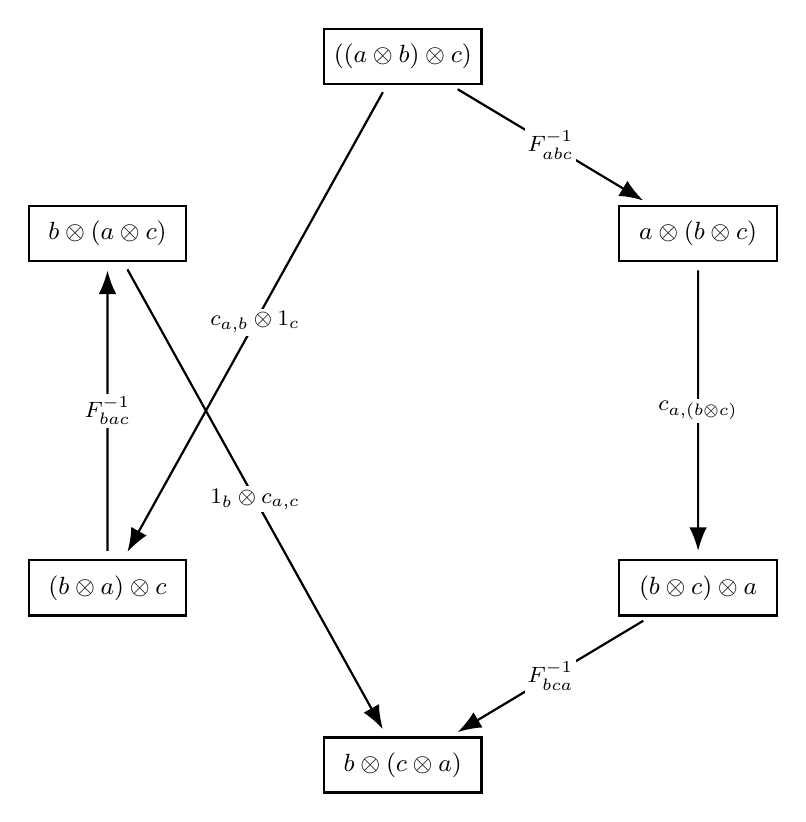
\begin{tikzpicture}[
    thick, 
    scale=1.5, 
    node distance=2.5cm, 
    state/.style={rectangle, draw, minimum width=2cm, minimum height=0.7cm, font=\small, align=center},
    arrow_label/.style={midway, fill=white, font=\footnotesize, inner sep=1pt}
]

    % Define nodes for the hexagon vertices
    \node[state] (s1) at (0, 3) {$((a \otimes b) \otimes c)$};
    \node[state] (s2) at (2.5, 1.5) {$a \otimes (b \otimes c)$};
    \node[state] (s3) at (2.5, -1.5) {$(b \otimes c) \otimes a$};
    \node[state] (s4) at (0, -3) {$b \otimes (c \otimes a)$};
    \node[state] (s5) at (-2.5, -1.5) {$(b \otimes a) \otimes c$};
    \node[state] (s6) at (-2.5, 1.5) {$b \otimes (a \otimes c)$};

    % Draw arrows and labels for the first hexagon identity (relating to $c_{a,b \otimes c}$)
    % Path 1: F then c then F
    \draw[-{Latex[length=3mm]}, shorten >=3pt, shorten <=3pt] (s1) -- (s2) node[arrow_label] {$F_{abc}^{-1}$};
    \draw[-{Latex[length=3mm]}, shorten >=3pt, shorten <=3pt] (s2) -- (s3) node[arrow_label] {$c_{a, (b \otimes c)}$};
    \draw[-{Latex[length=3mm]}, shorten >=3pt, shorten <=3pt] (s3) -- (s4) node[arrow_label] {$F_{bca}^{-1}$};

    % Path 2: c then F then c
    \draw[-{Latex[length=3mm]}, shorten >=3pt, shorten <=3pt] (s1) -- (s5) node[arrow_label] {$c_{a,b} \otimes 1_c$};
    \draw[-{Latex[length=3mm]}, shorten >=3pt, shorten <=3pt] (s5) -- (s6) node[arrow_label] {$F_{bac}^{-1}$};
    \draw[-{Latex[length=3mm]}, shorten >=3pt, shorten <=3pt] (s6) -- (s4) node[arrow_label] {$1_b \otimes c_{a,c}$};

\end{tikzpicture}
\end{document}
